\chapter{Production \& Site Services}
\section{Team Structure}
The Site Services and Production team was composed of Bx Muller, Imke Hoffmann, Will Tuffrey, Alex Jones, Keith Turner and Bob Todd with lots of support from Millie Burgh, Woodcraft Folk Events Assistant. Support was also given by a number of individuals at camp, including Huw Hickman. \\

This sized team worked well for a Venturer Camp sized event. There were a number of volunteers who were unable to commit much before camp, however they took on considerable sized roles at camp. 
\subsection{Roles Within The Team}
Bx, Imke and Millie led on Site Services \& Production in the run up to camp; while Keith and Bob focused on their specialities, stage and electricity respectively. Millie focused on booking infrastructure, including the marquee and porta-loos as well as procurement of some supplies from suppliers in advance of camp. \\

The role of sorting Village Kit initially lay with Millie, was then passed to Thomas (Camp Coordinator) and finally to Bx. This caused some confusion between team members about who was responsible for what, especially as camp got closer and we were working out how to divide up the Village's kit. \\

On site during the camp, Huw, Will, Alex and Imke worked together on the Site Services. Huw, Will and Alex led on gas while Imke focused on Camp Hygiene - primarily toilets and showers.  \\

During camp, Mike, Rick and Alex (Biblins Staff Team) also provided support with the site's infrastructure. This was extremely helpful as they know much more about the site than any of the Venturer Camp team!
\subsection{Evaluation of Team Structure}
The team felt that there was a lot of work, especially before the camp. This is something that the team wasn't prepared for however with support from the Camp Coordinator and Woodcraft Folk Events Assistant, they made work. Will and Alex felt they had to adapt their roles from what they were expecting it to be to what it actually became on site. \\

The team felt that not having a leader was a disadvantage as there wasn't a single person having oversight of all aspects of Site Services and Production. They recommended that this person should have a comprehensive knowledge of camp operations. The team also felt that there was a need for a clear distinction between ``people who know'' and ``people who do'', as this would enable younger people to be upskilled in Site Services \& Production roles, without having to agree to coordinate the whole thing!\\

On site, Bx took on an advisory role rather than boots on the ground with the Site Services team role due to leadership commitments with her local group. This caused a lack of continuity between the pre-camp planning and the on-site operations.\\ 

The team felt that the Central Clan worked very well and that it is something which should be repeated at future events. Central Clan was a daily working party with no particular purpose advertised. This meant it could take on whatever tasks were needed on that particular day, most commonly - cleaning the toilets which were not cleaned by Biblin's cleaner. 

\section{Supporting Events}
\subsection{Pre-Camp}
The team had mixed experiences with their online pre-camp session. Most didn't attend their session which left the person leading it to have a stressful experience. It's suggested that alternative volunteers should be found to facilitate sessions with team leaders there to answer questions and provide information.\\

A very small number of the team attended the On-Site Pre-Camp, with all team members commenting that it would have been useful for the entire team to attend. Bob found it helpful to meet the team in person and work out the site layout, something which was fundamental to the success of the Camp Radio.
\subsection{Working Week}
Bob and Keith both attended working week, no one else from the team was able to make it. It was felt that having some of the Site Services team there would have been beneficial.
\subsection{Takedown}
Members of the team stayed during takedown for as long as they were required for. This worked out to be only a single day, due to their excellent preparations during camp for takedown. As already discussed in the Takedown section earlier in this report, it would have been useful to have additional help, especially with the physical side of this role. 

\section{On-Camp Operations}
\subsection{Daily Structure}
On-Camp, the team's day would often involve attending their village's circle, managing the central clan then addressing issues as they arise. For the gas team, they were busy around meal times when KPs ran out of gas. 
\subsection{Support}
Team members were able to take time off during the day, and all members were able to take a day off due to the team's size. The team felt well-supported by the coordinator and Volunteer Support, despite the fact that the team members weren't all aware of PEB. It was suggested that better communication around the purpose of PEB would benefit future events. 

\section{Site Services \& Production Specific Insights}
The team expressed the need for better preparation \& communications. Keith and Bob enjoyed the experience and appreciated the support. For all team members, it was recommended to have a bike as the site is pretty expansive and the role covers the whole of the site! 
\subsection{Technical \& Stage Services}
Keith provided all the technical equipment from his personal stores. We hired a 7x3.5m Steel Deck stage from Stage Lighting Services at 1m high. It was found that the stage was too high for the height of the marquee we had, as the performers couldn't stand up all the way at the far edges. A 0.6m or 0.7m high stage would have sufficed. \\

Keith found it worked well to train up a couple of Venturers on DJing, sound and lighting control throughout the week. On the last night - they were left to do it and they did an excellent job!\\

Keith appreciated the height of the stage as he was able to store the majority of bulky equipment under it or within a small store tent he pitched at the rear of the main marquee. Small, valuable equipment (including microphones and laptops) were stored in his car. 

\subsection{Signs}
A task completed during Working Week was creating all the signs for centres and central points of interest. This task was completed by the Concordia Volunteer team using thin white-coated plywood and marker pens. Millie oversaw this process to ensure the right signs were being produced.\\

In advance of camp, signs for priority seating and hazard warning signs for gas storage locations were digitally designed then printed and laminated. A priority seat was provided in each centre as well as at strategic points along the path. These were appreciated and well used. The chairs which were used had stiff upper backs.
\subsection{Toilets}
Venturer Camp used all the toilets on the site, including the Western and Eastern Toilet Blocks and the Bunkhouse Toilet Block. 6 additional porta-loos were also hired, providing additional toilet capacity in the central area and at the far-eastern end of the site adjacent to Elysium Village. This worked very well, with enough capacity for all campers.\\

Codes for the toilets were distributed on the first day to villages with the instruction that villages should give their members the codes to their closest toilet block to them. This worked well. The porta-loos were padlocked shut during Working Week as they were dropped off a few days before camp started and we wanted to prevent members of the public using them. This worked, however it would help to have the padlocks on site before the porta-loos arrived as we had to go and buy them. Signs were posted on the porta-loos instructing members of the public not to use them and where they could find a public toilet on site.  \\

The Eastern and Western toilet block was cleaned by the Biblin's cleaner, who was contracted for 6 days a week during the camp as it was peak summer season. This had mixed reviews. The Site Services Team were pleased that they didn't have to clean the toilets however for the cleaner's safety \& ease, the entire block is closed while they are working. This caused issues as Venturers disregarded the signs and used the toilet blocks while the cleaner was working. The cleaner reported these issues to the Coordinator and a message got out to villages the following morning which prevented further issues surrounding this. Knowing about the block closure in the future would allow better communication around this. \\

One other incident of note within the Toilet Blocks was a Gender Neutral Protest. Due to an administrative oversight, we had not de-gendered any of the main toilet blocks, leaving the only truly Gender Neutral facilities as the Porta-Loos and the Western Toilet Block. Some young people decided to protest against this at the Eastern Toilet block which caused some confusion, however it was dealt with. For future events, it would be recommended to de-gender more toilets as we did not create a truly inclusive and welcoming environment.\\

Toilet Paper was used at a rate of around 1.3 rolls per person per week. This is higher than what we had expected it to be. The Site Services team managed stock levels well and ensured that a shopping trip was done to a local cash \& carry to purchase more when required, before we ran out. Enough toilet paper was left at the end of the event to provide for Takedown and leave some at Biblins.
\subsection{Showers}
The showers on site were situated within Biblin's East and West toilet blocks. These worked fine, with little-to-no maintenance required from the Site Services team. Participants found that the facilities weren't the best, however they're perfectly good showers which is all you need!\\

It was found that when run for a long time, they lightly flood the toilet block floors. There's nothing we could have done about this as by design that's what they do. It's worth the Site Services team being on hand to mop out if they get too wet however.\\

We didn't have any shower related incidents like we have had at previous events, which the Site Services team appreciated.
\subsection{Central Provision of Consumables}
The Site Services team were responsible for provisioning some catering consumables for each village. This was a limited amount of washing up liquid and other cleaning supplies. There was confusion over whether we should be doing this or not, given we were providing kitchen stuff however consumables are a grey area. Attendees have requested clearer communication around this for future events.

\subsection{Central Clan}
The Site Services \& Production team ran Central Clan each day, which was a working party that could be assigned to any needed task. The team ran it as they would meet the clans from the 5 villages and split them into smaller groups, giving them tasks to get on with. This worked well and motivated villages to keep the toilets near them clean.\\

It was commented that villages would appreciate knowledge of activities such as this further in advance so that it can be factored into rotas etc.

\subsection{Waste \& Recycling}
With Biblins being an already established camp-site, the waste \& recycling situation is already very well established. Additional collections were organised to take place during Venturer Camp which managed the amount of waste very well. The only time that the bins were badly overflowing was during Takedown, which is expected. A shuffle of bin bags completed by the site team rectified this very quickly.\\

Biblins has two types of bins: mixed recycling and general waste. This is un-ideal for obvious reasons however it was not feasible for us to do anything about it at this event. For future events, it may have been worth exploring possibilities of local farmers who may have been able to take food waste or paying for a van to take glass to a Local Authority Waste Centre. \\

In addition to the additional empties during camp, it would be helpful in the future to have an empty on the morning of arrivals day. From the groups camping before Venturer Camp began, some of the bins were already quite full which led to a slight challenge.\\

The Central Clan tasks also included litter picks. The Site Services team will need a stock of litter pickers \& PPE for this, something we were unable to source. Villages also need clear instructions that they need to leave their pitch in an acceptable condition as one village failed to do so, they may also benefit from support in planning their groups exit. The village who left their pitch in a mess had a large proportion of their campers who had to leave very early in the morning, leaving a small team left to pack up everything and get it in the van; which was an impossible task. 

\subsection{Central Tent}
Getting a Main Marquee for Venturer Camp proved quite difficult. Two bookings were cancelled before we found a local company (County Marquees, based out of Chepstow) who were able to supply us with a SIZE at short notice. Their service was excellent and they were of great value.\\

The remainder of the Central tents were sourced from stores at Biblins itself. Four centres were situated within 5x10m marquees from Common Ground, with two more used for Stewards HQ / Info Point and for the Site Services tent. The Media Centre used the West Coventry Kitchen Tent, from the Common Ground store room. The Radio Station, Cinema Tent and Safe Space tent were all sourced from the basement of the Bunkhouse.\\

The main food depot proved a large challenge to source as we needed a substantially sized tent which we could logistically transport to and from Biblins. We explored a number of possibilities before settling on using New Barnet's main marquee. This was supported by a small store tent (used for Fridges \& Cool boxes) and the `Sea Change' Marquee from the Bunkhouse Basement Stores. 

\subsection{Village Equipment}
During the idea conceptualisation stages of the project, it was decided that the central team would organise village equipment themselves, rather than expecting each village to be self-sufficient. The reason for this was to simplify the administration each village would need to do, with regards to working out equipment and to hopefully reduce the amount of equipment needed to travel around the country.\\

There was lots of back and forth between districts and the central team, and unfortunately due to different people in communications at different times - the goalposts for districts provided kit changed. The initial conversations were had in late 2022, then with no communication until early summer 2023. This caused some districts to think that we no longer needed their kit, and as such volunteers were no longer available to support the transport of it. \\

In the end, we used the following:
\begin{itemize}
    \item Oxford provided a village's marquee, 2 kitchen tents and a full kitchen's worth of equipment. A van was hired and used to transport the equipment to and from site and the van stayed on site for the duration of Venturer Camp with the driver \& van available should it be required.
    \item New Barnet provided a kitchen's worth of equipment alongside their marquee which was used for the Food Depot and an events shelter. They also provided a large number of tables \& benches which were distributed throughout the site. A 2-van convoy was used to get the equipment to site during Working Week; and the kitchen equipment was returned after camp with the large marquee being returned on the night of Friday 11 August.
    \item Heightate \& Holloway provided a marquee and some tables and benches. This arrived before Venturer Camp for their District camp and the smaller items were stored in the Bunkhouse Kitchen. It was all transported back to Heighgate \& Holloway during Takedown. 
    \item Lewisham \& Greenwich provided a full village's worth of equipment. They were camping on Pitches 6 \& 7 for their district camp the week before camp, which meant their pitch allocation for their village was planned carefully to ensure they didn't have to move everything. Their equipment was transported via their van, arriving for their district camp and leaving on Sunday 13 August, after their van had been used for Ealing's kit the day before. 
    \item Hackney provided a full village's worth of equipment (minus marquee). They were camping on Pitch 6 \& 7 the week before Lewisham \& Greenwich were. They stored their equipment (minus Marquee, see below) in a store tent on the boundary of Pitches 7 \& 8, as they would be on pitch 8 for Venturer Camp. This worked well, however some additional administration was required to ensure this worked! 
    \item Stroud provided their large marquee to Hackney to use for their District Camp and then for a village at Venturer Camp. This was erected on Pitch 7 and left up for the duration of Hackney and Lewisham \& Greenwich district camp then for Venturer Camp. This meant that the Lewisham \& Greenwich marquee was used in Dinas Affaraon due to its ability to be moved where as the Stroud marquee stayed in Camelot. The marquee was transported via Hackney's van, arriving for Hackney's district camp and leaving on Saturday 12 August.
    \item Ealing provided a full village's worth of equipment. Adam Senior drove Tom Brook's van to Ealing on Friday 4 August before camp to collect the equipment. At the end of camp, it was returned to Ealing on Saturday 12 August by Tom Brooks in his van.
\end{itemize}

\begin{figure}[ht]
    \centering
    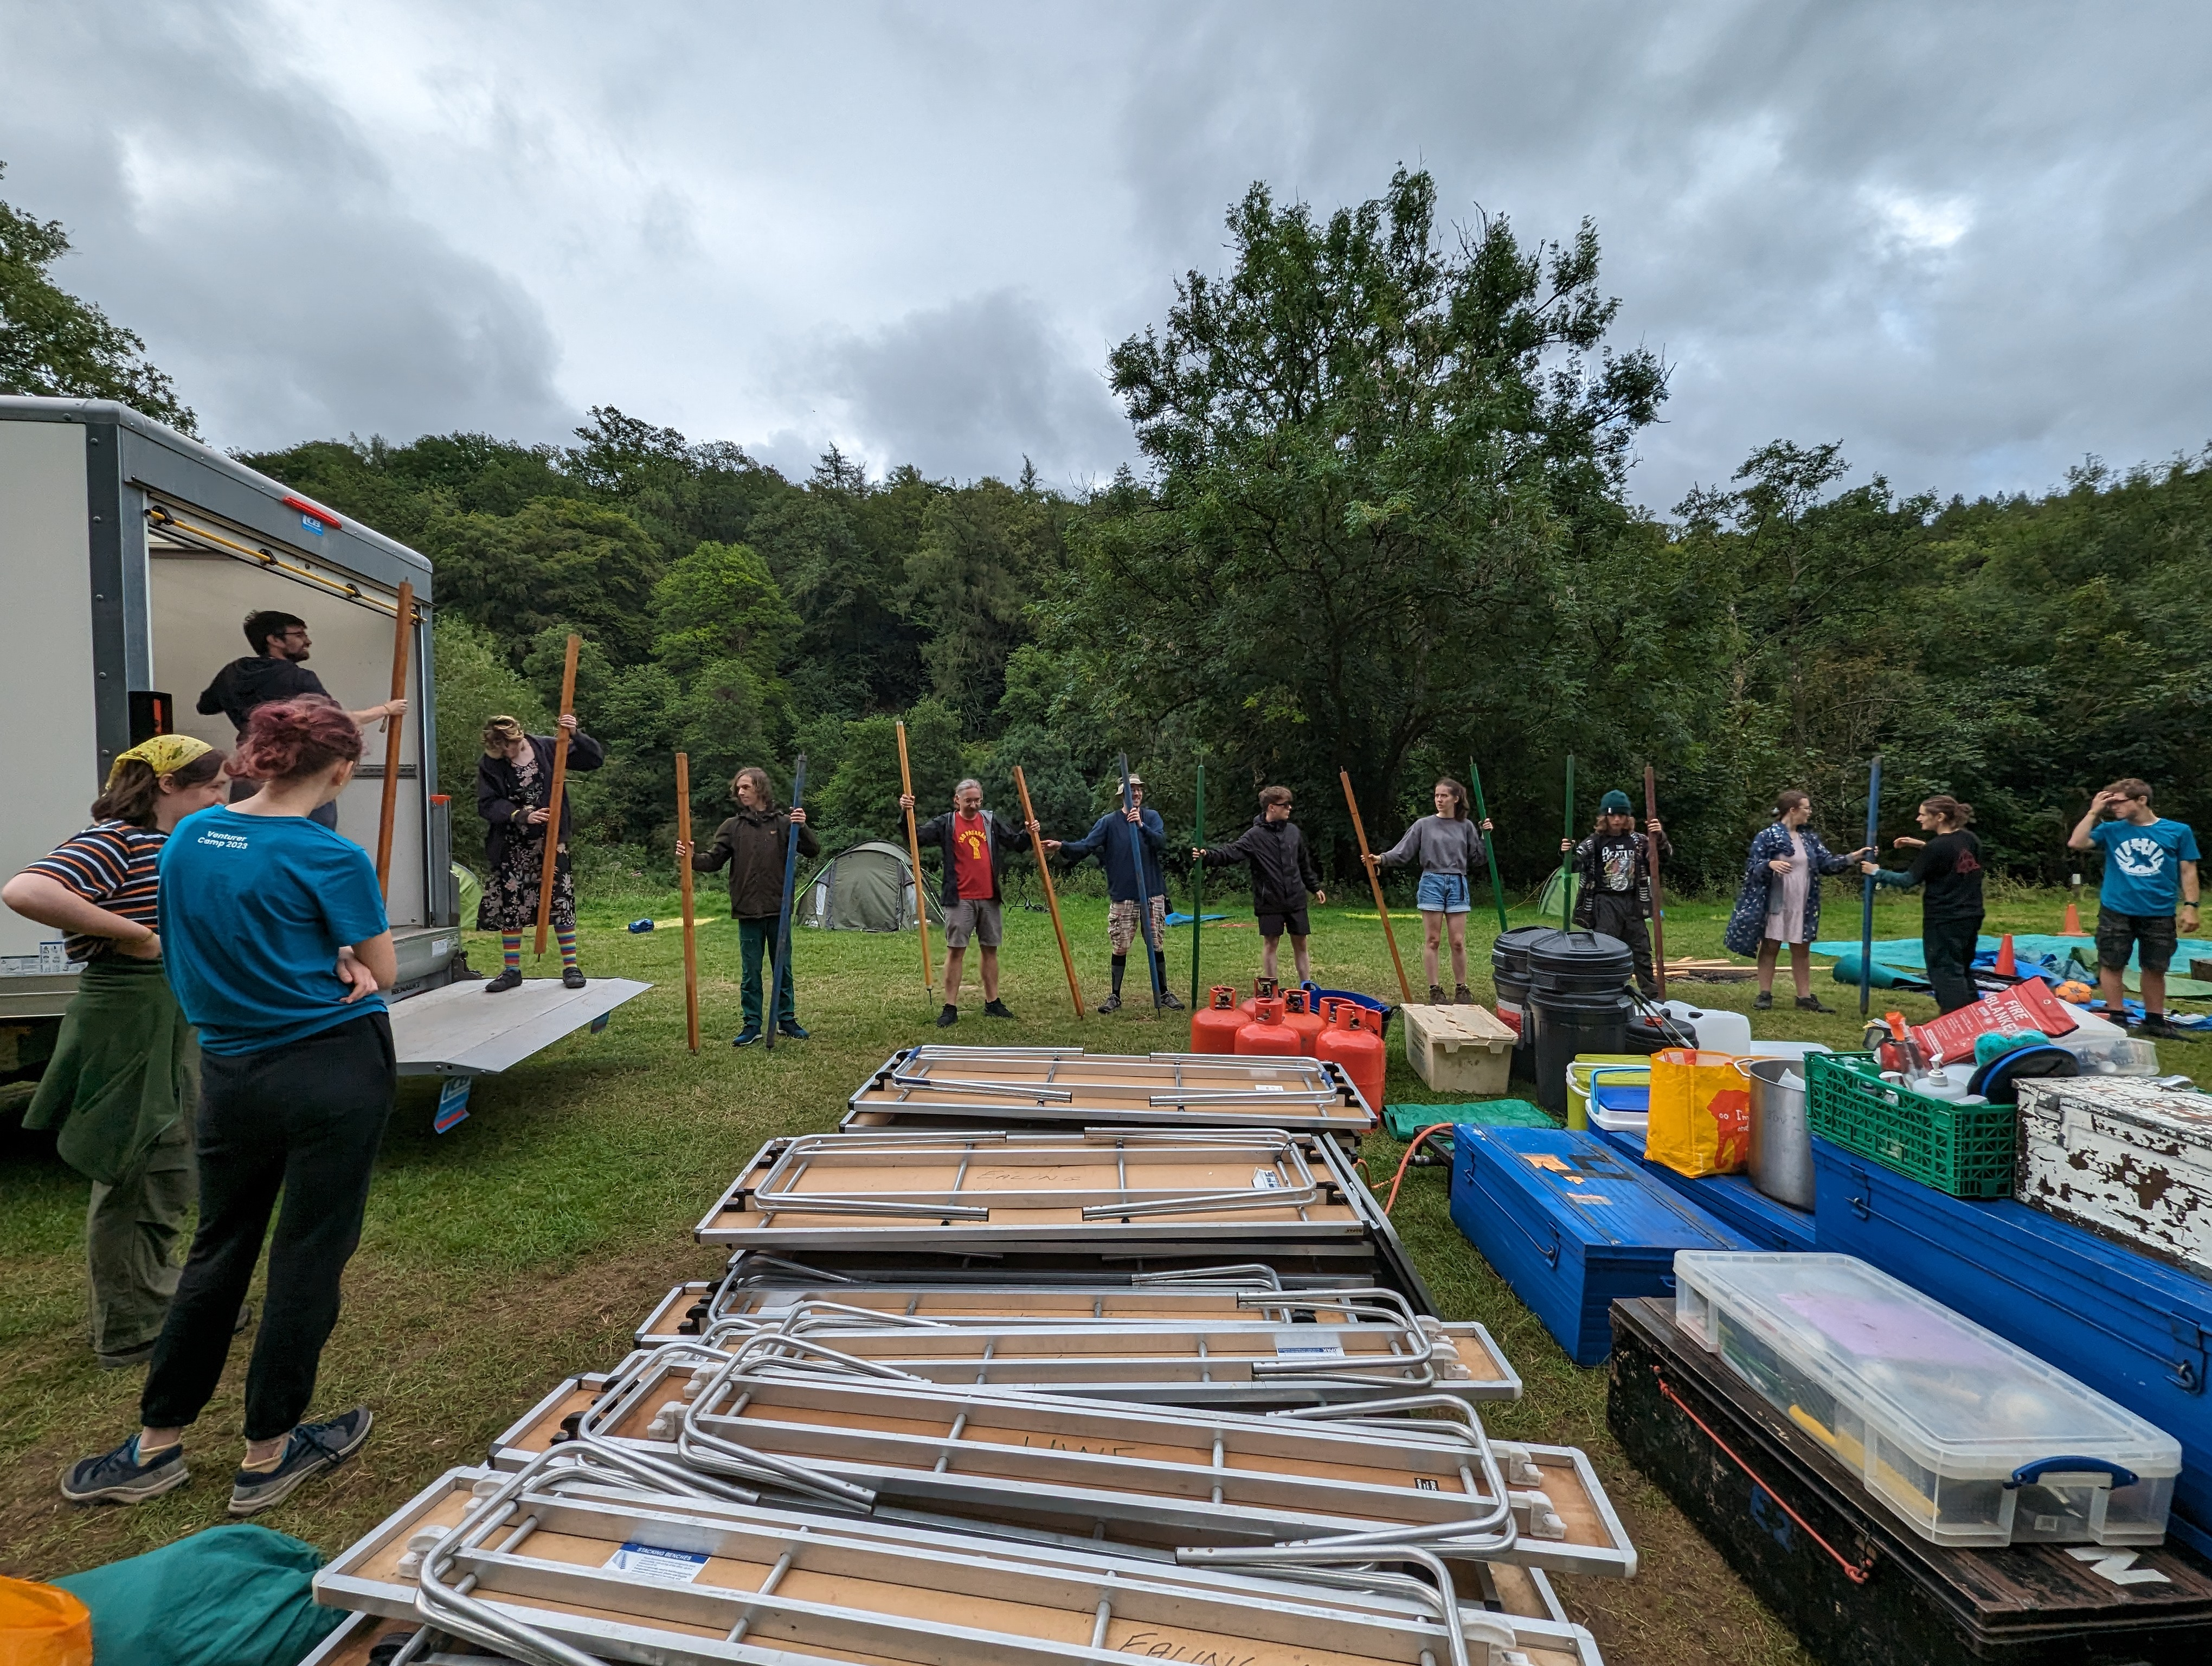
\includegraphics[width=0.8\textwidth]{assets/van-loading-rs.jpg}
    \caption{Elysium loading their van at the end of camp (\textit{RS})}
\end{figure}

Despite all these different districts providing equipment, some was still required from Biblins' stores and some was traded between districts for the duration of camp. \\

Overall, logistics headaches aside - this system worked. The core budget included funds to reimburse districts for van hire for use of their equipment which worked well. There were no major breakages of equipment or damages. Groups coming to Venturer Camp were grateful that equipment was sourced for them. Despite some of the challenges in solving the equipment logistics, it would be recommended to repeat this process for future Venturer Camps; larger events would need more consideration as to the feasibility of it. \\

The component of providing equipment which caused a major logistical problem was tables and benches for Villages. When discussing with districts what they could and couldn't provide, and what was within legal weight limits for a Luton van, we had omitted to discuss tables and benches. When we went back to districts in Summer 2023, it turned out that the districts were not able to provide as many tables and benches as we had hoped they could. This ended up with New Barnet providing tables and benches for almost the entire central area and two villages. This part was definitely too much of a headache for the sized team we had and we should have hired the required equipment as tables and benches don't cost excessive amounts to hire. 

\subsection{Electricity}
We had to build the support framework for the PV panels, then wire up the 24 volt battery / inverter system. Paul Fleming brought the Leicester solar trailer too, which was integrated into the system, and provided the Power Station tent. All together, we had about 3.7kWp of solar input, and about 15kWh of storage. Power was distributed at 230V 50Hz, with centre-tap earth.  \\


Safety  is obviously  an important concern. The main hazards are electric shock, burns/fire, and trips. These were minimised by earth leakage  (RCCBs) on all feeds, multiple safety earths, appropriate fusing and overcurrent trips, limiting access to the batteries and their connections, and by routing distribution cables away  from walkways,  in cable protectors or overhead. All mains voltage connectors/devices were well off the ground, or in water proof protection, in case of local flooding. \\


All the central area tents were provided with lighting, and around 200 metres of fairy lights were installed. These were mostly sourced from the stocks in the Common Ground room of the Bunkhouse.\\


The cinema was well used. It had a 250W projector, and a very efficient 100W power  amp for sound, and showed 2 or 3 films per day.\\


The Radio Station uses very little power, but is quite time consuming to set up, with it's 3 battery powered micro transmitters needed to persuade the signal around the massive bend in the Biblins valley.  It seemed to have a reasonable audience, but we don't  have an accurate measure of that.\\


Bob was kept pretty busy  during the camp keeping all this stuff working well, checking power consumption, and making additions / mending things where needed.
